%%%%%%%%%%%%%%%%%
% From Template %
%%%%%%%%%%%%%%%%%

\documentclass[%
class=scrreprt,
chapterprefix=false,%
open=right,%
twoside=false,%
paper=a4,%
logofile={Logo\_zentral\_farbig\_EN.png},%
thesistype=master,%
UKenglish,%
]{se2thesis}
\listfiles
\usepackage[ngerman,main=UKenglish]{babel}
\usepackage{blindtext}
\usepackage[%
csquotes=true,%
booktabs=true,%
siunitx=true,%
minted=true,%
selnolig=true,%
widowcontrol=false,%
microtype=true,%
% biblatex=true,%
cleveref=true,%
]{se2packages}

% Own change (from Lisa)
% Changing citeauthor to use et el.
\usepackage[maxcitenames=2,backend=biber]{biblatex}
% End own change

\begin{filecontents}{\jobname.bib}
	@article{linaker2015guidelines,
		author = {Linåker, Johan and Sulaman, Sardar and Host, Martin and de Mello, Rafael},
		year = {2015},
		month = {05},
		pages = {},
		title = {Guidelines for Conducting Surveys in Software Engineering}
	}
	
	@article{boehm2001defect,
		title={Defect reduction top 10 list},
		author={Boehm, Barry and Basili, Victor R},
		journal={Computer},
		volume={34},
		number={1},
		pages={135--137},
		year={2001}
	}
	
	@article{buse2009learning,
		title={Learning a metric for code readability},
		author={Buse, Raymond PL and Weimer, Westley R},
		journal={IEEE Transactions on software engineering},
		volume={36},
		number={4},
		pages={546--558},
		year={2009},
		publisher={IEEE}
	}
	
	@inproceedings{aggarwal2002integrated,
		title={An integrated measure of software maintainability},
		author={Aggarwal, Krishan K and Singh, Yogesh and Chhabra, Jitender Kumar},
		booktitle={Annual Reliability and Maintainability Symposium. 2002 Proceedings (Cat. No. 02CH37318)},
		pages={235--241},
		year={2002},
		organization={IEEE}
	}
	
	@inproceedings{fakhoury2019improving,
		title={Improving source code readability: Theory and practice},
		author={Fakhoury, Sarah and Roy, Devjeet and Hassan, Adnan and Arnaoudova, Vernera},
		booktitle={2019 IEEE/ACM 27th International Conference on Program Comprehension (ICPC)},
		pages={2--12},
		year={2019},
		organization={IEEE}
	}
	
	@article{scalabrino2018comprehensive,
		title={A comprehensive model for code readability},
		author={Scalabrino, Simone and Linares-V{\'a}squez, Mario and Oliveto, Rocco and Poshyvanyk, Denys},
		journal={Journal of Software: Evolution and Process},
		volume={30},
		number={6},
		pages={e1958},
		year={2018},
		publisher={Wiley Online Library}
	}
	
	@inproceedings{posnett2011simpler,
		title={A simpler model of software readability},
		author={Posnett, Daryl and Hindle, Abram and Devanbu, Premkumar},
		booktitle={Proceedings of the 8th working conference on mining software repositories},
		pages={73--82},
		year={2011}
	}
	
	@inproceedings{dorn2012general,
		title={A General Software Readability Model},
		author={Jonathan Dorn},
		year={2012}
	}
	
	@inproceedings{scalabrino2017automatically,
		title={Automatically assessing code understandability: How far are we?},
		author={Scalabrino, Simone and Bavota, Gabriele and Vendome, Christopher and Linares-V{\'a}squez, Mario and Poshyvanyk, Denys and Oliveto, Rocco},
		booktitle={2017 32nd IEEE/ACM International Conference on Automated Software Engineering (ASE)},
		pages={417--427},
		year={2017},
		organization={IEEE}
	}
	
	@inproceedings{daka2015modeling,
		title={Modeling readability to improve unit tests},
		author={Daka, Ermira and Campos, Jos{\'e} and Fraser, Gordon and Dorn, Jonathan and Weimer, Westley},
		booktitle={Proceedings of the 2015 10th Joint Meeting on Foundations of Software Engineering},
		pages={107--118},
		year={2015}
	}
	
	@article{mi2022towards,
		title={Towards using visual, semantic and structural features to improve code readability classification},
		author={Mi, Qing and Hao, Yiqun and Ou, Liwei and Ma, Wei},
		journal={Journal of Systems and Software},
		volume={193},
		pages={111454},
		year={2022},
		publisher={Elsevier}
	}
	
	@inproceedings{mi2018gamification,
		title={A gamification technique for motivating students to learn code readability in software engineering},
		author={Mi, Qing and Keung, Jacky and Mei, Xiupei and Xiao, Yan and Chan, WK},
		booktitle={2018 International Symposium on Educational Technology (ISET)},
		pages={250--254},
		year={2018},
		organization={IEEE}
	}
	
	@article{mi2018improving,
		title={Improving code readability classification using convolutional neural networks},
		author={Mi, Qing and Keung, Jacky and Xiao, Yan and Mensah, Solomon and Gao, Yujin},
		journal={Information and Software Technology},
		volume={104},
		pages={60--71},
		year={2018},
		publisher={Elsevier}
	}
	
	@book{brooks1987no,
		title={No silver bullet},
		author={Brooks, Frederick and Kugler, H},
		year={1987},
		publisher={April}
	}
	
	@article{loriot2022styler,
		title={Styler: learning formatting conventions to repair Checkstyle violations},
		author={Loriot, Benjamin and Madeiral, Fernanda and Monperrus, Martin},
		journal={Empirical Software Engineering},
		volume={27},
		number={6},
		pages={149},
		year={2022},
		publisher={Springer}
	}
	
	@inproceedings{yasunaga2020graph,
		title={Graph-based, self-supervised program repair from diagnostic feedback},
		author={Yasunaga, Michihiro and Liang, Percy},
		booktitle={International Conference on Machine Learning},
		pages={10799--10808},
		year={2020},
		organization={PMLR}
	}
	
	@inproceedings{xu2019method,
		title={Method name suggestion with hierarchical attention networks},
		author={Xu, Sihan and Zhang, Sen and Wang, Weijing and Cao, Xinya and Guo, Chenkai and Xu, Jing},
		booktitle={Proceedings of the 2019 ACM SIGPLAN workshop on partial evaluation and program manipulation},
		pages={10--21},
		year={2019}
	}
	
	@inproceedings{allamanis2016convolutional,
		title={A convolutional attention network for extreme summarization of source code},
		author={Allamanis, Miltiadis and Peng, Hao and Sutton, Charles},
		booktitle={International conference on machine learning},
		pages={2091--2100},
		year={2016},
		organization={PMLR}
	}
	
	@article{hestness2017deep,
		title={Deep learning scaling is predictable, empirically},
		author={Hestness, Joel and Narang, Sharan and Ardalani, Newsha and Diamos, Gregory and Jun, Heewoo and Kianinejad, Hassan and Patwary, Md Mostofa Ali and Yang, Yang and Zhou, Yanqi},
		journal={arXiv preprint arXiv:1712.00409},
		year={2017}
	}
	
	@inproceedings{liu2019learning,
		title={Learning to spot and refactor inconsistent method names},
		author={Liu, Kui and Kim, Dongsun and Bissyand{\'e}, Tegawend{\'e} F and Kim, Taeyoung and Kim, Kisub and Koyuncu, Anil and Kim, Suntae and Le Traon, Yves},
		booktitle={2019 IEEE/ACM 41st International Conference on Software Engineering (ICSE)},
		pages={1--12},
		year={2019},
		organization={IEEE}
	}
	
	@article{deimel1985uses,
		title={The uses of program reading},
		author={Deimel Jr, Lionel E},
		journal={ACM SIGCSE Bulletin},
		volume={17},
		number={2},
		pages={5--14},
		year={1985},
		publisher={ACM New York, NY, USA}
	}
	
	@inproceedings{raymond1991reading,
		title={Reading source code.},
		author={Raymond, Darrell R},
		booktitle={CASCON},
		volume={91},
		pages={3--16},
		year={1991}
	}
	
	@article{rugaber2000use,
		title={The use of domain knowledge in program understanding},
		author={Rugaber, Spencer},
		journal={Annals of Software Engineering},
		volume={9},
		number={1-4},
		pages={143--192},
		year={2000},
		publisher={Springer}
	}
	
	@article{likert1932technique,
		title={A technique for the measurement of attitudes.},
		author={Likert, Rensis},
		journal={Archives of psychology},
		year={1932}
	}
	
	@inproceedings{wyrich2019towards,
		title={Towards an autonomous bot for automatic source code refactoring},
		author={Wyrich, Marvin and Bogner, Justus},
		booktitle={2019 IEEE/ACM 1st international workshop on bots in software engineering (BotSE)},
		pages={24--28},
		year={2019},
		organization={IEEE}
	}
	
	@article{pawlak2016spoon,
		title={Spoon: A library for implementing analyses and transformations of java source code},
		author={Pawlak, Renaud and Monperrus, Martin and Petitprez, Nicolas and Noguera, Carlos and Seinturier, Lionel},
		journal={Software: Practice and Experience},
		volume={46},
		number={9},
		pages={1155--1179},
		year={2016},
		publisher={Wiley Online Library}
	}
	
	@article{someoliayi2022sorald,
		title={Sorald: Automatic Patch Suggestions for SonarQube Static Analysis Violations},
		author={Someoliayi, Khashayar Etemadi and Harrand, Nicolas Yves Maurice and Larsen, Simon and Adzemovic, Haris and Phu, Henry Luong and Verma, Ashutosh and Madeiral, Fernanda and Wikstrom, Douglas and Monperrus, Martin},
		journal={IEEE Transactions on Dependable and Secure Computing},
		year={2022},
		publisher={IEEE}
	}
	
	@inproceedings{allamanis2015suggesting,
		title={Suggesting accurate method and class names},
		author={Allamanis, Miltiadis and Barr, Earl T and Bird, Christian and Sutton, Charles},
		booktitle={Proceedings of the 2015 10th joint meeting on foundations of software engineering},
		pages={38--49},
		year={2015}
	}
	
	@article{alon2019code2vec,
		title={code2vec: Learning distributed representations of code},
		author={Alon, Uri and Zilberstein, Meital and Levy, Omer and Yahav, Eran},
		journal={Proceedings of the ACM on Programming Languages},
		volume={3},
		number={POPL},
		pages={1--29},
		year={2019},
		publisher={ACM New York, NY, USA}
	}
	
	@article{chicco2020advantages,
		title={The advantages of the Matthews correlation coefficient (MCC) over F1 score and accuracy in binary classification evaluation},
		author={Chicco, Davide and Jurman, Giuseppe},
		journal={BMC genomics},
		volume={21},
		number={1},
		pages={1--13},
		year={2020},
		publisher={BioMed Central}
	}
	
	@article{dubay2004principles,
		title={The principles of readability.},
		author={DuBay, William H},
		journal={Online Submission},
		year={2004},
		publisher={ERIC}
	}
	
	@book{klare1964measurement,
		location = {Ames},
		title = {The measurement of readability},
		pagetotal = {328},
		publisher = {Iowa State University Press},
		author = {Klare, George R.},
		date = {1963},
		keywords = {Bibliographies, Bibliography, Readability (Literary style)},
	}
	
	@article{tashtoush2013impact,
		title={Impact of programming features on code readability},
		author={Tashtoush, Yahya and Odat, Zeinab and Alsmadi, Izzat M and Yatim, Maryan},
		year={2013}
	}
	
	@inproceedings{sedano2016code,
		title={Code readability testing, an empirical study},
		author={Sedano, Todd},
		booktitle={2016 IEEE 29th International conference on software engineering education and training (CSEET)},
		pages={111--117},
		year={2016},
		organization={IEEE}
	}
	
	@article{tashtoush2013impact,
		title={Impact of programming features on code readability},
		author={Tashtoush, Yahya and Odat, Zeinab and Alsmadi, Izzat M and Yatim, Maryan},
		year={2013}
	}
	
	@inproceedings{oliveira2020evaluating,
		title={Evaluating code readability and legibility: An examination of human-centric studies},
		author={Oliveira, Delano and Bruno, Reydne and Madeiral, Fernanda and Castor, Fernando},
		booktitle={2020 IEEE International Conference on Software Maintenance and Evolution (ICSME)},
		pages={348--359},
		year={2020},
		organization={IEEE}
	}
	
	@article{mi2023graph,
		title={A graph-based code representation method to improve code readability classification},
		author={Mi, Qing and Zhan, Yi and Weng, Han and Bao, Qinghang and Cui, Longjie and Ma, Wei},
		journal={Empirical Software Engineering},
		volume={28},
		number={4},
		pages={87},
		year={2023},
		publisher={Springer}
	}
	
	@article{mi2021effectiveness,
		title={The effectiveness of data augmentation in code readability classification},
		author={Mi, Qing and Xiao, Yan and Cai, Zhi and Jia, Xibin},
		journal={Information and Software Technology},
		volume={129},
		pages={106378},
		year={2021},
		publisher={Elsevier}
	}
	@book{martin2009clean,
		title={Clean code: a handbook of agile software craftsmanship},
		author={Martin, Robert C},
		year={2009},
		publisher={Pearson Education}
	}
	@book{wilson2007beautiful,
		title={Beautiful code: Leading programmers explain how they think},
		author={Wilson, Greg and Oram, Andy},
		year={2007},
		publisher={" O'Reilly Media, Inc."}
	}
	@book{beck2007implementation,
		title={Implementation patterns},
		author={Beck, Kent},
		year={2007},
		publisher={Pearson Education}
	}
	@article{alawad2019empirical,
		title={An empirical study of the relationships between code readability and software complexity},
		author={Alawad, Duaa and Panta, Manisha and Zibran, Minhaz and Islam, Md Rakibul},
		journal={arXiv preprint arXiv:1909.01760},
		year={2019}
	}
	@inproceedings{mannan2018towards,
		title={Towards understanding code readability and its impact on design quality},
		author={Mannan, Umme Ayda and Ahmed, Iftekhar and Sarma, Anita},
		booktitle={Proceedings of the 4th ACM SIGSOFT International Workshop on NLP for Software Engineering},
		pages={18--21},
		year={2018}
	}
	@inproceedings{johnson2019empirical,
		title={An empirical study assessing source code readability in comprehension},
		author={Johnson, John and Lubo, Sergio and Yedla, Nishitha and Aponte, Jairo and Sharif, Bonita},
		booktitle={2019 IEEE International conference on software maintenance and evolution (ICSME)},
		pages={513--523},
		year={2019},
		organization={IEEE}
	}
	@article{xia2017measuring,
		title={Measuring program comprehension: A large-scale field study with professionals},
		author={Xia, Xin and Bao, Lingfeng and Lo, David and Xing, Zhenchang and Hassan, Ahmed E and Li, Shanping},
		journal={IEEE Transactions on Software Engineering},
		volume={44},
		number={10},
		pages={951--976},
		year={2017},
		publisher={IEEE}
	}
	@article{segedinac2024assessing,
		title={Assessing code readability in Python programming courses using eye-tracking},
		author={Segedinac, Milan and Savi{\'c}, Goran and Zeljkovi{\'c}, Ivana and Slivka, Jelena and Konjovi{\'c}, Zora},
		journal={Computer Applications in Engineering Education},
		volume={32},
		number={1},
		pages={e22685},
		year={2024},
		publisher={Wiley Online Library}
	}
	@article{ribeiro2018attributes,
		title={Attributes influencing the reading and comprehension of source code--discussing contradictory evidence},
		author={Ribeiro, Talita Vieira and Travassos, Guilherme Horta},
		journal={CLEI Electronic Journal},
		volume={21},
		number={1},
		pages={5--1},
		year={2018}
	}
	@inproceedings{mi2018inception,
		title={An inception architecture-based model for improving code readability classification},
		author={Mi, Qing and Keung, Jacky and Xiao, Yan and Mensah, Solomon and Mei, Xiupei},
		booktitle={Proceedings of the 22nd International Conference on Evaluation and Assessment in Software Engineering 2018},
		pages={139--144},
		year={2018}
	}
	@inproceedings{sharma2020egan,
		title={EGAN: An Effective Code Readability Classification using Ensemble Generative Adversarial Networks},
		author={Sharma, Shashank and Srivastava, Sumit},
		booktitle={2020 International Conference on Computation, Automation and Knowledge Management (ICCAKM)},
		pages={312--316},
		year={2020},
		organization={IEEE}
	}
	@article{choi2020metric,
		title={Metric and tool support for instant feedback of source code readability},
		author={Choi, Sangchul and Park, Sooyong and others},
		journal={Tehni{\v{c}}ki vjesnik},
		volume={27},
		number={1},
		pages={221--228},
		year={2020},
		publisher={Faculty of Mechanical Engineering in Slavonski Brod; Faculty of Electrical~…}
	}
	@article{choi2020metric,
		title={Metric and tool support for instant feedback of source code readability},
		author={Choi, Sangchul and Park, Sooyong and others},
		journal={Tehni{\v{c}}ki vjesnik},
		volume={27},
		number={1},
		pages={221--228},
		year={2020},
		publisher={Faculty of Mechanical Engineering in Slavonski Brod; Faculty of Electrical~…}
	}
	@inproceedings{mi2022enhanced,
		title={An enhanced data augmentation approach to support multi-class code readability classification},
		author={Mi, Qing and Hao, Yiqun and Wu, Maran and Ou, Liwei},
		booktitle={International conference on software engineering and knowledge engineering},
		year={2022}
	}
	@inproceedings{vitale2023using,
		title={Using Deep Learning to Automatically Improve Code Readability},
		author={Vitale, Antonio and Piantadosi, Valentina and Scalabrino, Simone and Oliveto, Rocco},
		booktitle={2023 38th IEEE/ACM International Conference on Automated Software Engineering (ASE)},
		pages={573--584},
		year={2023},
		organization={IEEE}
	}
	@inproceedings{mi2022rank,
		title={Rank Learning-Based Code Readability Assessment with Siamese Neural Networks},
		author={Mi, Qing},
		booktitle={Proceedings of the 37th IEEE/ACM International Conference on Automated Software Engineering},
		pages={1--2},
		year={2022}
	}
	@article{mi2023makes,
		title={What makes a readable code? A causal analysis method},
		author={Mi, Qing and Chen, Mingjie and Cai, Zhi and Jia, Xibin},
		journal={Software: Practice and Experience},
		volume={53},
		number={6},
		pages={1391--1409},
		year={2023},
		publisher={Wiley Online Library}
	}
\end{filecontents}
\addbibresource{\jobname.bib}

\usepackage{hyperref}

\author{Lukas Krodinger}
\title{Advancing Code Readability: Mined \& Modified Code for Dataset Generation}
\degreeprogramme{M.Sc. Computer Science}
\matrnumber{89801}
\supervisor{Prof. Dr. Gordon Fraser}
%\external{Prof.~John Doe,~PhD}
\advisor{Lisa Griebl}
\department{Faculty of Computer Science and Mathematics}
\institute{Chair of Software Engineering II}
\location{Passau}


%%%%%%%%%%%%%%%%%%%%%%
% Installed Packages %
%%%%%%%%%%%%%%%%%%%%%%
% For java code embeddings
\usepackage{color}
\definecolor{dkgreen}{rgb}{0,0.6,0}
\definecolor{gray}{rgb}{0.5,0.5,0.5}
\definecolor{mauve}{rgb}{0.58,0,0.82}

\usepackage{listings}
\lstset{frame=tb,
	language=Java,
	aboveskip=3mm,
	belowskip=3mm,
	showstringspaces=false,
	columns=flexible,
	basicstyle={\small\ttfamily},
	showstringspaces=true,
	numbers=none,
	numberstyle=\tiny\color{gray},
	keywordstyle=\color{blue},
	commentstyle=\color{dkgreen},
	stringstyle=\color{mauve},
	breaklines=true,
	breakatwhitespace=true,
	tabsize=3
}

% Start counting of chapters with 1
\usepackage{chngcntr}
\counterwithout{chapter}{section}
\counterwithin{chapter}{part}
\renewcommand{\thesection}{\arabic{section}}
\renewcommand{\thechapter}{\arabic{chapter}.0}

% Footnotes
\newcounter{urlfootnote}
\newcommand{\onecurl}[2]{%
	\stepcounter{urlfootnote}%
	\expandafter\def\csname urlfootnote:#1\endcsname{\theurlfootnote}%
	\footnote{\label{url:#1}\url{#1}, accessed: #2}%
}
\usepackage{etoolbox}
\newcommand{\curl}[2]{%
	\ifcsdef{urlfootnote:#1}{%
		\textsuperscript{\ref{url:#1}}%
	}{%
		\onecurl{#1}{#2}%
	}%
}

% Indentation of "Assumption 1" etc. in enumerate
\usepackage{enumitem}

% Nice skips between paragraphs
\usepackage{parskip} 

\begin{document}
	
	\frontmatter
	
	\maketitle
	
	\begin{abstract}
		% TODO: Rework once work is done
		This work presents an innovative method for generating datasets intended for code readability classification in the context of a master's thesis. We offer a comprehensive overview of code readability, delving into existing classifiers that consider both manually crafted and automatically extracted code readability features. Furthermore, we summarize existing datasets of manually annotated Java code snippets.
		
		The core contribution of this work lies in the introduction of an automatic data generation technique, alongside a dataset produced using this methodology. Our approach relies on the extraction and modification of code snippets sourced from public GitHub repositories. Notably, our dataset significantly surpasses the scale of any previously available dataset designed for readability classification.
		
		To evaluate the newly generated dataset, we conducted a user survey and train a state of the art code readability classification model, both with and without the integration of the new dataset. This analysis aims to assess the quality of our new dataset and the effectiveness of the generation approach employed.

	\end{abstract}
	
	\mainmatter
	
	\tableofcontents
	
	\section{Introduction} \label{Introduction}
	In the realm of software development, the significance of code readability cannot be overstated. Together with understandability, it serves as the foundation for efficient collaboration, comprehension, and maintenance of software systems~\cite{posnett2011simpler, aggarwal2002integrated}. 
	Maintenance alone will consume over 70\% of the total lifecycle cost of a software product and for maintenance, the most time-consuming act is reading code~\cite{buse2009learning, deimel1985uses, rugaber2000use, boehm2001defect}.
	Therefore, it is important to ensure a high readability of code. In order to archive this, we need to measure readability.
	
	In the last years, researchers have proposed several metrics and models for assessing code readability with an accuracy of up to 81.8\%~\cite{buse2009learning, posnett2011simpler, dorn2012general, daka2015modeling}. In recent years, deep learning based models are able to achieve an accuracy of up to 85.3\%~\cite{mi2018improving, mi2022towards}.
	However, these models do not capture what developers think of readability improvements~\cite{fakhoury2019improving}. This suggests that there is room for improvement in readability classification of source code. 
	
	% TODO: Add Sections ref
	% Background and related work
	In the following sections we will clarify what source code readability is. We will summarize background knowledge for both classical and deep learning based classification approaches. We will have a look at related work.
	
	% Dataset generation approach
	In section TODO we will explain our new dataset generation approach in detail. We will SUBSECTIONS
	
	% Readability Classification model
	After introducing our new dataset we will evaluate it based on a user study and a state of the art readability classification model in section TODO. Based on the dataset, the user study and the model we will propose our research questions.
	
	% Evaluation
	We will then answer our research questions based on results of the survey and model performance in section TODO.
	
	% Discussion
	We will show possible threads to the dataset generation approach and our evaluation and discuss them in section TODO.
	
	% Conclusion
	In the last section we summarize our work, draw conclusions from it and propose future work.
	
	\section{Background and related work} \label{Background and related work}
	In the following sections you find an overview over background and related work regarding code readability and our dataset generation approach.
	
	\subsection{Code Readability} \label{Readability}
	To properly discuss readability, in particular readability of source code we first define this term. There are various differing definitions for code readability:
	
	% Readability in general
	\citeauthor{klare1964measurement} defines readability in general as “the ease of understanding or comprehension due to the style of writing.” 
	% TODO: More citations
	%https://files.eric.ed.gov/fulltext/ED490073.pdf
	%	 This definition focuses on writing
	%	style as separate from issues such as content, coherence, and organization. In a
	%	similar manner, Gretchen Hargis and her colleagues at IBM (1998) state that
	%	readability, the “ease of reading words and sentences,” is an attribute of clarity.
	%	The creator of the SMOG readability formula G. Harry McLaughlin (1969)
	%	defines readability as: “the degree to which a given class of people find certain
	%	reading matter compelling and comprehensible.” This definition stresses the
	%	interaction between the text and a class of readers of known characteristics such
	%	as reading skill, prior knowledge, and motivation.
	%	Edgar Dale and Jeanne Chall’s (1949) definition may be the most
	%	comprehensive: “The sum total (including all the interactions) of all those
	%	elements within a given piece of printed material that affect the success a group
	%	of readers have with it. The success is the extent to which they understand it,
	%	read it at an optimal speed, and find it interesting.” 
	%	\cite{dubay2004principles}
	
	% Definiton
	\citeauthor{buse2009learning} states regarding code readability: "We define readability as a human judgment of how easy a
	text is to understand."

	% Definition
	\citeauthor{tashtoush2013impact} combines multiple other aspects from various definitions to their definition of code readability:
	\begin{enumerate}
		\item Ratio between lines of code and number of commented lines
		\item Writing to people not to computers
		\item Making a code locally understandable without searching for declarations and definitions
		\item Average number of right answers to a series of questions about a program in a given length of time
	\end{enumerate}	
	However, this results in a long and complex definition.
	
	\citeauthor{scalabrino2018comprehensive} says, that it is a subjective concept that is influenced by a number of factors, including the complexity of code, the usage of design concepts, the formatting of code, source code lexicon, and the visual aspects of the code.
	
	% Definition
	Recent definitions of code readability are shorter, trying to focus on the key aspects. \citeauthor{oliveira2020evaluating} defines readability as "what makes a program easier or harder to read and apprehend by developers".
			
	% Definition
	Also \citeauthor{mi2021effectiveness} summarizes code readability as "a human judgment of how easy a piece of
	source code is to understand". This is again close to the definition of \citeauthor{buse2009learning}.
	
	% Related terms	
	However, there are various related terms to readability: Understandability, usability, reusability, complexity, and maintainability \citeauthor{tashtoush2013impact}. 
	
	Readability is not the same as complexity. Complexity is an “essential” property of software that arises
	from system requirements, while readability is an “accidental” property that is not determined by the problem statement~\cite{buse2009learning, brooks1987no}.
	
	Previous definitions are close to understandability.
	
	\citeauthor{scalabrino2018comprehensive} defines aspects of understandability: "Complexity, usage of design concepts, formatting, source code lexicon, and visual aspects (e.g., syntax highlighting) have been widely recognized as elements that impact program understanding" \cite{martin2009clean, wilson2007beautiful, beck2007implementation}.
	
	\citeauthor{posnett2011simpler} states that readability is the syntactic aspect of processing code, while understandability is the semantic aspect.
	
	Based on \citeauthor{posnett2011simpler}, \citeauthor{scalabrino2018comprehensive} says about readability: "Readability measures the effort of the developer to access the information contained in the code, while understandability measures the complexity of such information."
	
	Readability is a human judgment of how easy a program source code is to read and comprehend \cite{buse2008evaluating, sedano2016code}. It is concerned with the syntactic aspects of code, such as the use of meaningful variable names, consistent formatting, and clear commenting.
	
	Understandability is the ability to grasp the meaning of a program source code and how it works \cite{oliveira2020evaluating, posnett2011simpler}. It is concerned with the semantic aspects of code, such as the underlying logic and the use of design patterns.
	
	For example, a developer can find a piece of code readable but still difficult to understand.
	Recent research gives evidence that there is no correlation between understandability and readability~\cite{scalabrino2017automatically}.	
	
	
	% However, \citeauthor{scalabrino2018comprehensive} also states, that "code readability remains to be a very subjective concept".
		
	%	
	%	For now we stick with the definition of BUSE and WEIMER which also \citeauthor{mi2023graph} sticks with:
	%	Code readability is defined as a measure of how easily developers can read and understand
	%	the source code (Buse and Weimer 2010; Lee et al 2013)
	%	% TODO: Continue

	Comparing the definitions of code readability in literature one can see, that there are some common aspects in most definitions. Those are:
	"ease/complexity of understanding/comprehension/apprehension", "human judgement" as well as the differentiation to understandability.
	Based on this, we come up with the following definition:
	Code Readability is a human judgment of the effort it takes to read and understand code. % , considering factors like style and structure.
	
	% Importance	
	Now that we have a grasp of what code readability refers to, let's take a brief look at the question, why code readability is important.
	In the domain of software development, the importance of code readability cannot be emphasized enough. Alongside understandability, it forms the basis for effective collaboration, comprehension, and maintenance of software systems~\cite{posnett2011simpler, aggarwal2002integrated}.
	It is a critical aspect of software quality, significantly influencing the maintainability, reusability, portability, and reliability of the source code \cite{alawad2019empirical, sedano2016code}. Poorly readable code increases the risk of introducing bugs \cite{mannan2018towards, scalabrino2018comprehensive} and can lead to higher costs during subsequent software maintenance and development \cite{johnson2019empirical}. On the other hand, readable code allows developers to identify and rectify bugs more easily \cite{mi2023graph}.
	Recent studies indicate that developers spend nearly 58\% of their time reading and comprehending source code~\cite{buse2009learning, deimel1985uses, rugaber2000use, boehm2001defect, tashtoush2013impact, sedano2016code, xia2017measuring}.
	%	In the field of software development, a major focus continues to be on code readability and its profound impact on these aspects, as confirmed by numerous studies~\cite{deimel1985uses, rugaber2000use, boehm2001defect, aggarwal2002integrated, posnett2011simpler, buse2009learning, tashtoush2013impact, sedano2016code, xia2017measuring, mannan2018towards, scalabrino2018comprehensive, alawad2019empirical, johnson2019empirical, mi2023graph}.
	Therefore, it is important to ensure a high readability of code. In order to archive this, we need to measure readability.
	
	In the last years, researchers have proposed several metrics and models for assessing code readability with an accuracy of up to 81.8\%~\cite{buse2009learning, posnett2011simpler, dorn2012general, daka2015modeling}. In recent years, deep learning based models are able to achieve an accuracy of up to 85.3\%~\cite{mi2018improving, mi2022towards}.
	However, these models do not capture what developers think of readability improvements~\cite{fakhoury2019improving}. This suggests that there is room for improvement in readability classification of source code.
	
%	% Importance
%	In software engineering, the terms readability, legibility, understandability, and comprehensibility have overlapping meanings. For example, Buse and Weimer [22] define “readability
%	as a human judgment of how easy a text is to understand”.
%	In a similar vein, Almeida et al. [23] affirm that “legibility is
%	fundamental to code maintenance; if source code is written
%	in a complex way, understanding it will require much more
%	effort”. In addition, Lin and Wu [24] state that ““Software
%	understandability” determines whether a system can be understood by other individuals easily, or whether artifacts of
%	one system can be easily understood by other individuals”.
%	Xia et al. [25] treat comprehension and understanding as
%	synonyms, expressing that “Program comprehension (aka.,
%	program understanding, or source code comprehension) is a
%	process where developers actively acquire knowledge about a
%	software system by exploring and searching software artifacts,
%	and reading relevant source code and/or documentation”.\cite{oliveira2020evaluating}
%	
%	% Importance
%	Software developers read code all the time. The very first step in each software evolution and
%	maintenance task is to carefully read and understand the code; this step needs to be done even
%	when the maintainer is the author of the code. Developers spend much time reading code, far more
%	than writing it from scratch [1]. Therefore, if code is readable, it is pretty easy to start changing it;
%	instead, modifying unreadable code is like assembling a piece of furniture with instructions written
%	in a foreign language the one does not speak: the task is not impossible, but difficult, and a few
%	screws still may remain unused.
%	Furthermore, incremental change [2, 3, 4], which is required to perform concept location, impact
%	analysis, and the corresponding change implementation/propagation, needs a prior code reading
%	step before it can take place. This is why “readable code” is a fundamental and highly desirable at
%	any stage during software maintenance and evolution.\cite{scalabrino2018comprehensive}
%	
%	% Definition
%	Readability vs understandability
%	t et al. [9] compared the difference between readability and understandability to the difference
%	between syntactic and semantic analysis. Readability measures the effort of the developer to access
%	the information contained in the code, while understandability measures the complexity of such
%	information. We defined a set of textual features that still capture aspects of code related to the
%	difficulty of accessing the information contained in a snippet. For example, NOC estimates the
%	number of concepts implemented in a snippet. A snippet with a few concepts, potentially more
%	readable, can still be hard to understand if a few concepts are not easy to understand. In our opinion,
%	textual features, which do not take into account semantics, like the ones we defined, can be used to
%	measure readability
%	\cite{scalabrino2018comprehensive}
%	
%	% Related terms
%	Definitions show clearly
%	that such quality attribute is related to some other attributes such as: understandability,
%	usability, reusability, complexity, or maintainability. 
%	Code readability is usually connected with comments and naming standards. While
%	those are two major factors that impact readability, there are also some other aspects to
%	consider.
%	One of the new concepts that appear in relation with software quality and readability
%	is the refactoring process. It means changing code structure externally without affecting
%	internal behavior to improve readability, flexibility, and enable easier modifications
%	[12-14]. Refactoring often aims to add new non functional objectives for code, without
%	affecting its main purpose by testing the code frequently.
%	In [15] the author defines “improving code readability” as the first advantage for
%	code refactoring. The survey briefly explains code refactoring techniques such as: field
%	encapsulation, type generalization, or methods renaming. Refactoring advantages
%	include: improving readability, maintainability, less complexity, and reusability.
%	\cite{tashtoush2013impact}

%
%	% Definition
%	In software engineering, the terms readability, legibility, understandability, and comprehensibility have overlapping meanings. For example, Buse and Weimer [22] define “readability
%	as a human judgment of how easy a text is to understand”.
%	In a similar vein, Almeida et al. [23] affirm that “legibility is
%	fundamental to code maintenance; if source code is written
%	in a complex way, understanding it will require much more
%	effort”. In addition, Lin and Wu [24] state that ““Software
%	understandability” determines whether a system can be understood by other individuals easily, or whether artifacts of
%	one system can be easily understood by other individuals”.
%	Xia et al. [25] treat comprehension and understanding as
%	synonyms, expressing that “Program comprehension (aka.,
%	program understanding, or source code comprehension) is a
%	process where developers actively acquire knowledge about a
%	software system by exploring and searching software artifacts,
%	and reading relevant source code and/or documentation”.\cite{oliveira2020evaluating}
%	
	

		
	
	
	
	% New, check and extend (Bard)
	%	Code readability is a human judgment of how easy a program source code is to understand \cite{buse2008evaluating}. It is a subjective concept that is influenced by a number of factors, including the complexity of the code, the usage of design concepts, the formatting of the code, the source code lexicon, and the visual aspects of the code \cite{scalabrino2018comprehensive}.
		

	
%	There are a number of different definitions of code readability in the literature. Some of these definitions are:
%	
%	"Code readability is the ease of understanding a program source code." \cite{buse2008evaluating}
%	"Code readability is the ratio between lines of code and number of commented lines." \cite{sedano2016code}
%	"Code readability is writing to people, not to computers." \cite{oliveira2020evaluating}
%	"Code readability is making a code locally understandable without searching for declarations and definitions." \cite{oliveira2020evaluating}
%	"Code readability is the average number of right answers to a series of questions about a program in a given length of time." \cite{oliveira2020evaluating}
%	While these definitions vary, they all share the common theme of measuring how easy it is for humans to understand the code.
%			
	
	
	%	% Old:
	%	To improve readability classification, we need to capture what readability is. We define readability as a subjective impression of the difficulty of code while trying to understand it~\cite{posnett2011simpler, buse2009learning}. Readability of code is a perceived barrier that needs to be overcome before it is possible to work with the code. The more readable code is, the lower the barrier~\cite{posnett2011simpler}.
	%	To give an example for high vs low readability, consider the code of listing~\ref{lst:cassandra-src-java-org-apache-cassandra-utils} from GitHub\curl{https://github.com/apache/cassandra/blob/trunk/src/java/org/apache/cassandra/utils/HeapUtils.java}{2023-25-07} and compare it to the code with the same functionality of listing~\ref{lst:cassandra-src-java-org-apache-cassandra-utils-modified}. You will notice that the first piece of code is more readable than the second one.
	%	
		
	%	There is another related term: understandability. Readability is the syntactic aspect of processing code, while understandability is the semantic aspect~\cite{posnett2011simpler}.
	%	For example, a developer can find a piece of code readable but still difficult to understand. Recent research gives evidence that there is no correlation between understandability and readability~\cite{scalabrino2017automatically}.	
	
%	\begin{listing}[!ht]
%		\begin{minted}[linenos, frame=lines, framesep=2mm]{java}
%			/**
%			* Logs the output of the specified process.
%			*
%			* @param p the process
%			* @throws IOException if an I/O problem occurs
%			*/
%			private static void logProcessOutput(Process p) throws IOException
%			{
%				try (BufferedReader input = new BufferedReader(new InputStreamReader(p.getInputStream())))
%				{
%					StrBuilder builder = new StrBuilder();
%					String line;
%					while ((line = input.readLine()) != null)
%					{
%						builder.appendln(line);
%					}
%					logger.info(builder.toString());
%				}
%			}
%		\end{minted}
%		\caption[An example for well readable code of the highly rated Cassandra GitHub repository]{An example for well readable code of the highly rated Cassandra GitHub repository \protect\footnotemark}
%		\label{lst:cassandra-src-java-org-apache-cassandra-utils}
%	\end{listing}
%	\footnotetext{\url{https://github.com/apache/cassandra/blob/trunk/src/java/org/apache/cassandra/utils/HeapUtils.java}, accessed: 2023-07-25}
	
	\begin{listing}[!ht]
		\begin{minted}[linenos, frame=lines, framesep=2mm]{java}
			/**
			* Logs the output of the specified process.
			*
			* @param p the process
			* @throws IOException if an I/O problem occurs
			*/
			private static void logProcessOutput(Process p) throws IOException
			{
				try (BufferedReader input = new BufferedReader(new InputStreamReader(p.getInputStream())))
				{
					StrBuilder builder = new StrBuilder();
					String line;
					while ((line = input.readLine()) != null)
					{
						builder.appendln(line);
					}
					logger.info(builder.toString());
				}
			}
		\end{minted}
		\caption[An example for well readable code of the highly rated Cassandra GitHub repository]{An example for well readable code of the highly rated Cassandra GitHub repository}
		\label{lst:cassandra-src-java-org-apache-cassandra-utils}
	\end{listing}
	
	\begin{listing}[!ht]
		\begin{minted}[linenos, frame=lines, framesep=2mm]{java}
			private 
				static 
			void 
			debug( Process 
			v1 
			)       throws IOException
			{
				// Doo debug
				try (BufferedReader   b 
				= new 
				BufferedReader(
				new InputStreamReader(
				v1.getInputStream()
				)
				)
				)
				{
					StrBuilder b2=new StrBuilder();String v2;while (null!=(v2=input.readLine())){b2.appendln(v2);} // Doo stuff
					m.info(  builder.toString()
					);
				}
			}
		\end{minted}
		\caption{The same example as in listing~\ref{lst:cassandra-src-java-org-apache-cassandra-utils} but modified to be poorly readable}
		\label{lst:cassandra-src-java-org-apache-cassandra-utils-modified}
	\end{listing}
	
%	\lstinputlisting[language=Java, firstline=8, lastline=26, caption={An example for highly readable code of the highly rated cassandra github repository},label={lst:cassandra-src-java-org-apache-cassandra-utils}]{cassandra-src-java-org-apache-cassandra-utils.java}
%	
%	\lstinputlisting[language=Java, firstline=8, lastline=29, caption={The same example modified to be poorly readable},label={lst:cassandra-src-java-org-apache-cassandra-utils-modified}]{cassandra-src-java-org-apache-cassandra-utils-modified.java}
	
	\subsection{Classical calculation approaches} \label{Classical calculation approaches}
	A first estimation for source code readability was the percentage of comment lines over total code lines~\cite{aggarwal2002integrated}. In the last years, researchers have proposed several more complex metrics and models for assessing code readability~\cite{buse2009learning, posnett2011simpler, dorn2012general, scalabrino2018comprehensive}.
	Those approaches used handcrafted features to calculate how readable a piece of code is. They were able to achieve up to 81.8\% accuracy in classification~\cite{scalabrino2018comprehensive}.
	
	\subsection{Deep Learning based approaches} \label{(Deep) Learning based approaches}
	More recent models use Deep Learning approaches in order to generate the features automatically. Those models have proven to be more accurate, achieving an accuracy of up to 85.3\%~\cite{mi2018improving, mi2022towards}.
	
	All the mentioned models were trained on the data of Buse, Dorn and Scalabrino consisting of in total 660 code snippets. The data was generated with surveys. They therefore asked developers several questions, including the question, how well readable the proposed source code is~\cite{buse2009learning, dorn2012general, scalabrino2018comprehensive}.
	
	\citeauthor{fakhoury2019improving} showed based on readability improving commit analysis that these models do not capture what developers think of readability improvements. They therefore analyzed 548 GitHub\curl{https://github.com/}{2023-07-25} commits manually. They suggest considering other metrics such as incoming method calls or method name fitting~\cite{fakhoury2019improving}.
	
	\subsection{Related work}
	\citeauthor{loriot2022styler} created a model that is able to fix Checkstyle\curl{https://checkstyle.org/}{2023-07-25} violations using Deep Learning. They inserted formatting violations based on a project specific format checker ruleset into code in a first step. They then used a LSTM neural network that learned how to undo those injections. Their approach is working on abstract token sequences. Their data is generated in a self-supervised manner~\cite{loriot2022styler}. A similar idea has been explored by \citeauthor{yasunaga2020graph}~\cite{yasunaga2020graph}. We will use the idea of intentional degradation of code for data generation.
	
	Another concept we will employ is from \citeauthor{allamanis2016convolutional}. They cloned the top open source Java projects on GitHub\curl{https://github.com/}{2023-07-25} for training a Deep Learning model. Those top projects were selected by taking the sum of the z-scores of the number of watchers and forks of each project. As the projects have thousands of forks and stars and are widely used among software developers, they can be assumed to be of high quality~\cite{allamanis2016convolutional}.
		
	% Related work
	\citeauthor{segedinac2024assessing} introduces a novel approach for code readability classification using eye-tracking data from 90 undergraduate students assessing Python code snippets.
	
	% Related work
	In a recent study participants demonstrated a consistent perception that Python code with more lines was deemed more comprehensible, irrespective of their level of experience. However, when it came to readability, variations were observed based on code size, with less experienced participants expressing a preference for longer code, while those with more experience favored shorter code. Both novices and experts agreed that long and complete-word identifiers enhanced readability and comprehensibility. Additionally, the inclusion of comments was found to positively impact comprehension, and a consensus emerged in favor of four indentation spaces \cite{ribeiro2018attributes}.
	
	% Related work
	\citeauthor{mi2018inception} introduces a novel approach, IncepCRM, for Code Readability Classification using deep learning, specifically based on the Inception architecture. Unlike traditional methods that rely on handcrafted features and various machine learning algorithms, IncepCRM automatically learns multi-scale features from source code with minimal manual intervention. The study empirically validates IncepCRM's performance with human annotator information as auxiliary input, demonstrating its superiority in accuracy compared to previous models across three publicly available datasets. The results confirm the feasibility and effectiveness of deep learning for code readability classification.
	
	% Related work
	Another study addresses concerns regarding the classification of code script readability by proposing a novel approach using Generative Adversarial Networks (GANs). Unlike previous studies relying on labor-intensive manual feature engineering, the proposed method involves encoding source codes into integer matrices with multiple granularities and utilizing an EGAN (Enhanced GAN) for code readability classification. The EGAN, comprising three GANs with identical architectures trained on differently preprocessed data, outperforms five state-of-the-art code readability models, achieving a quality increase ranging from 2\% to 15\%. This approach demonstrates the effectiveness of GANs in code readability classification tasks, providing a substantial improvement without the need for manual interface design \cite{sharma2020egan}.
	
	% Related work
	The paper of \citeauthor{choi2020metric} introduces an enhanced source code readability metric aimed at quantitatively measuring code readability in the software maintenance phase. The proposed metric achieves a substantial explanatory power of 75.74\%. Additionally, the authors developed a tool named Instant R. Gauge, integrated with Eclipse IDE, to provide real-time readability feedback and track readability history, allowing developers to gradually improve their coding habits. Experimental results indicate that methods authored using the proposed approach exhibit higher readability compared to those without it. The study concludes by highlighting the potential future contribution of Instant R. Gauge as an open-source project to assist developers in enhancing their source code readability.
	
	% Related work
	\citeauthor{mi2023graph}'s study addresses the importance of code readability in software development and introduces a novel graph-based representation method for code readability classification. The proposed method involves parsing source code into a graph with abstract syntax tree (AST), combining control and data flow edges, and converting node information into vectors. The model, comprising Graph Convolutional Network (GCN), DMoNPooling, and K-dimensional Graph Neural Networks (k-GNNs) layers, extracts syntactic and semantic features. Evaluation on a Java dataset demonstrates superior performance with 72.5\% and 88\% accuracy in three-class and two-class readability classification, respectively. The graph-based approach outperforms existing models, indicating its effectiveness in capturing code readability-related features. Future work includes overcoming dataset limitations, exploring heterogeneous graph methods, and improving model performance. 
	
	% Related work
	\citeauthor{mi2022enhanced}'s paper addresses the challenge of multi-class code readability classification, emphasizing the importance of code readability in software maintenance. Due to a scarcity of labeled data, most prior research focused on binary classification. The authors propose an enhanced data augmentation approach, incorporating domain-specific data transformation and Generative Adversarial Networks (GANs). Experimental results demonstrate a significant improvement of 6.3\%, reaching a state-of-the-art multi-class code readability classification accuracy of 68.0\% compared to using only the original data. The proposed method is proven effective, and future work aims to further enhance classifier performance by exploring alternative code representation methods, increasing the number of readability levels, and addressing the challenge of limited dataset size through additional labeling efforts.
	
	% Related work
	\citeauthor{vitale2023using}'s paper introduces a novel approach to automatically identify and suggest readability-improving actions for code snippets. The authors develop a methodology to identify readability-improving commits, creating a dataset of 122k commits from GitHub's revision history. They train the T5 model to emulate developers' actions in improving code readability, achieving a prediction accuracy between 21\% and 28\%. The empirical evaluation shows that 82-90.8\% of the dataset commits aim to improve readability, and the model successfully mimics developers in 21\% of cases. The dataset and scripts are released for further research. Future work includes refining the methodology, testing additional Language Model Models (LLMs), and extending the approach to other programming languages. The goal is to create a comprehensive tool for readability improvement.
	
	% Related work
	\citeauthor{mi2022rank}'s paper introduces a novel approach to code readability assessment by framing it as a learning-to-rank task. The proposed model employs siamese neural networks to rank code pairs based on their readability. The evaluation on three publicly available datasets demonstrates promising results, with an accuracy of 83.5\%, precision of 86.1\%, recall of 81.6\%, F-measure of 83.6\%, and AUC of 83.4\%. The research suggests that the approach effectively ranks code readability by comparing code pairs. However, the study acknowledges areas for improvement, such as addressing ties in readability levels, experimenting with different source code representations, exploring more sophisticated neural network architectures, and considering practical applications, such as detecting readability changes in version control systems to aid developers in monitoring code changes. 
	
	% Related work
	\citeauthor{mi2023makes}' paper aims to understand the causal relationship between code features and readability. To overcome potential spurious correlations, the authors propose a causal theory-based approach, utilizing the PC algorithm and additive noise models to construct a causal graph. The linear regression algorithm, based on the back-door criterion, is then employed to determine the causal effect of various features on code readability. Experimental results using human-annotated readability data reveal that the average number of comments positively impacts code readability, while the average number of assignments, identifiers, and periods has a negative impact. The proposed approach provides developers with insights into code readability patterns.
	
	% Related work
	\citeauthor{oliveira2020evaluating}'s study addresses the challenge of acquiring large datasets with manual labels for training deep learning models in code readability classification. To overcome this limitation, the authors propose data augmentation approaches to artificially increase the training set size, reducing the risk of overfitting and aiming to improve classification accuracy. They create transformed versions of code snippets by manipulating aspects such as comments, indentations, and names of classes/methods/variables, based on domain-specific knowledge. Additionally, they explore the use of Auxiliary Classifier GANs to generate synthetic data. Experimental results show a significant improvement in the classification performance of deep neural networks when trained on the augmented corpus, achieving a state-of-the-art accuracy of 87.38\%. The findings highlight the effectiveness of data augmentation in code readability classification. Future work involves extending the proposed approach systematically, exploring more ground-truth data, experimenting with other classifiers, and aiming for better performance with larger datasets and more complex deep learning models.
		
	
	 
	% TODO: Split content?	 
	\section{Dataset Generation Approach} \label{Dataset Generation Approach}
	\section{Readability Classification Model} \label{Readability Classification Model}

	
	We will investigate whether it is possible to score a higher accuracy as current models in classifying code readability for Java using Deep Learning. Therefore, we will train the model from \citeauthor{mi2022towards}~\cite{mi2022towards} with more data. We will consider augmenting the model with a method name classifier and incorporating semantic encoding for tabs and spaces. The training data will be generated in a novel way for classification of readability, inspired by \citeauthor{loriot2022styler}~\cite{loriot2022styler}. The method name classifier is similar to Code2Vec~\cite{alon2019code2vec}. The combination of all components is novel to the best of our knowledge. You can find a visualization of the planned modifications of \citeauthor{mi2022towards}'s model in figure~\ref{fig:model_pipeline}. We will focus on generating training data, as the approach will be usable for further research in the field of source code readability.
	
	\begin{figure}[t]
		\centering
		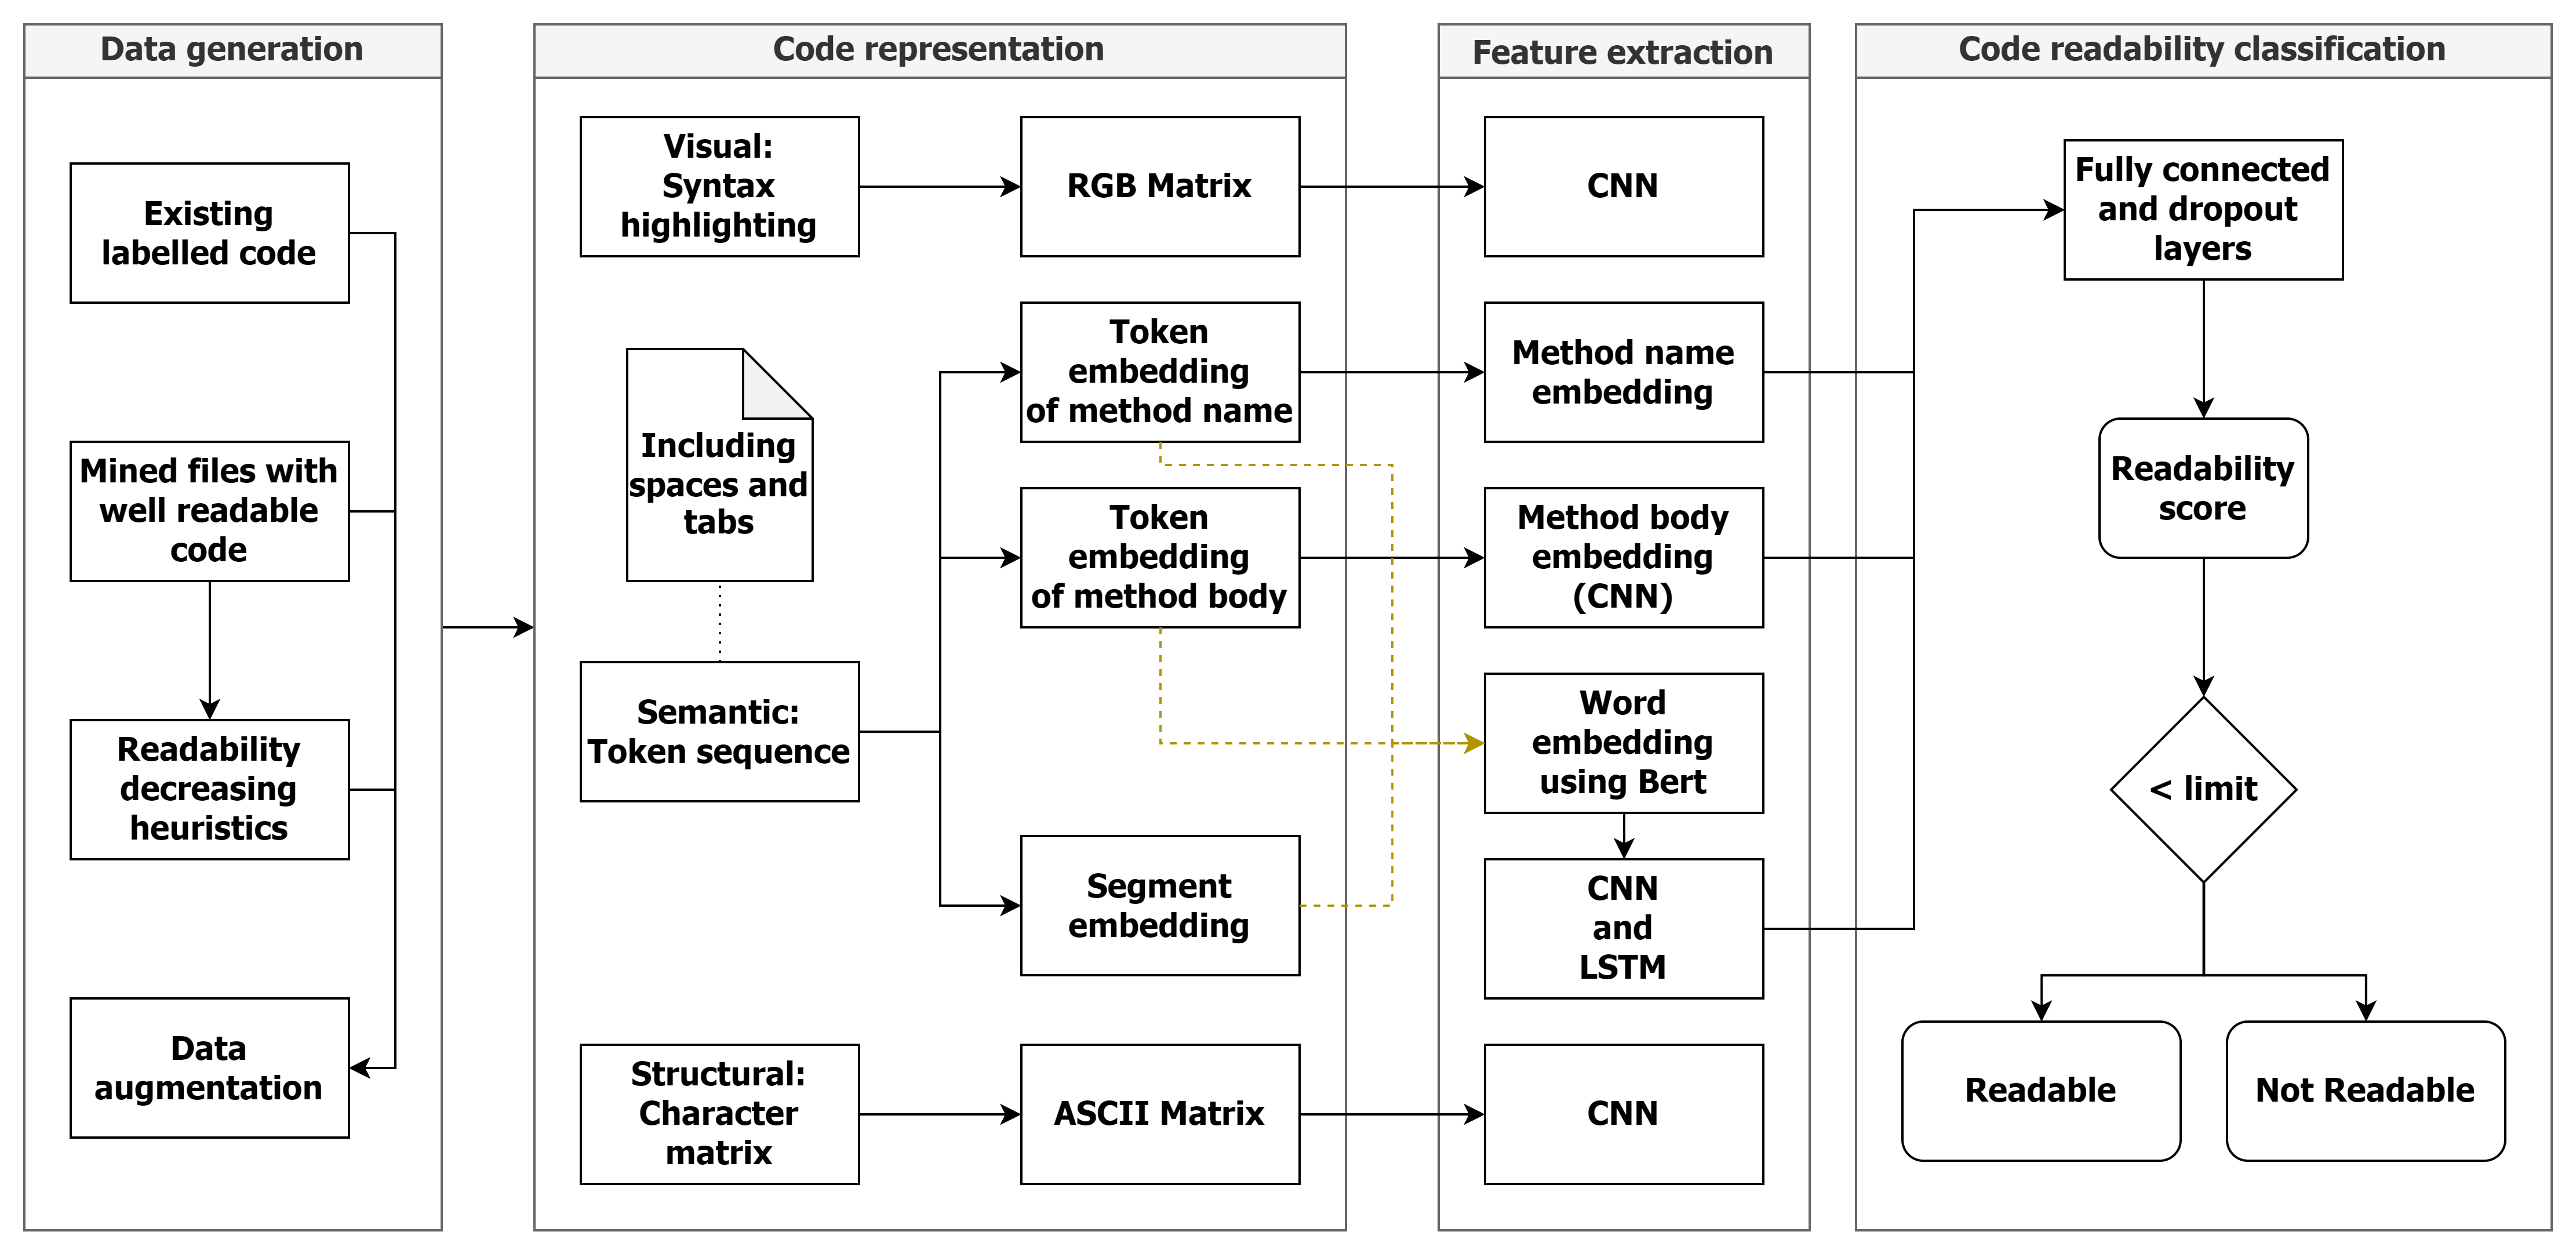
\includegraphics[width=\textwidth]{img/model_pipeline_old.png}
		\caption{Overview of the planned approach.}
		\label{fig:model_pipeline}
	\end{figure}
	
	% TODO: Inline this in research questions?
	% \subsection{Data generation} \label{Data generation}
	Deep Learning based models perform better the more training data they get~\cite{hestness2017deep}. Therefore, one approach in order to further improve existing models is to gather more training data.
	This requires, as it was done previously, a lot of effort and persons willing to rate code based on their readability. We present another approach for gathering training data.
	
	In a first step, GitHub repositories with known high code quality are downloaded and labeled as highly readable. We select repositories using a similar approach as \citeauthor{allamanis2016convolutional}~\cite{allamanis2016convolutional} and then assume that they contain only well readable code.
	In a second step, the code is manipulated so that it is subsequently less readable. This approach is similar to the approach of \citeauthor{loriot2022styler}~\cite{loriot2022styler}. After both steps, we have a new, automatically generated training dataset for source code readability classification.
		
	% Readabililty Decreasing Heuristics
	This brings up the question, how to manipulate code so that it is less readable afterwards. We therefore introduce a tool called Readability Decreasing Heuristics. As the name suggests this is a collection of heuristics that, when applied to source code, lower the readability of it. For example such a heuristic is to replace spaces with newlines. Another example is to increase the indentation of a code block by a tab or multiple spaces. Moreover, with most changes it is also possible to do exactly the opposite (replacing newlines with spaces, decreasing indentation), which in most cases also decreases the readability of source code.
	
	Code snippets in Java are syntactically the same, before and after applying Readability Decreasing Heuristics. Complexity did not change either. However, if various modifications are applied many times, those changes are capable of lowering the readability of source code, as the comparison of listing~\ref{lst:cassandra-src-java-org-apache-cassandra-utils} and listing~\ref{lst:cassandra-src-java-org-apache-cassandra-utils-modified} suggests.
	
	Note that we assume two things for the data generation approach:
	\begin{enumerate}[label={Assumption \arabic*},ref={\arabic*},leftmargin=*]
		\item \label{well-readable-assumption} \textbf{(well-readable-assumption)} The selected repositories contain only well-readable code.
		\item \label{poorly-readable-assumption} \textbf{(poorly-readable-assumption)} After applying Readability Decreasing Heuristics, the code is poorly readable.
	\end{enumerate}
	
	% Model modifications/Further improvements
	\label{model-modifications}
	In recent years it was shown that Deep Learning models can be further improved by modifying the structure of the architecture or by introducing new components, parts or layers to existing architectures. 
	We suggest two improvements for the model of \citeauthor{mi2022towards}~\cite{mi2022towards}. Firstly, we want to embed spaces and tabs as semantic tokens. Secondly, adding a method name fitting classifier as a component of the overall model could be an improvement.
	% Surpassing
	\label{suggestions}If there is time left, we will try to surpass the performance of recent source code readability classifiers with those improvements to data generation and the model.
	%, such as the model proposed by \citeauthor{mi2022towards}~\cite{mi2022towards}.
	
	% We suggest two improvements for the model of \citeauthor{mi2022towards}~\cite{mi2022towards}:
	%\begin{enumerate}
	%	\item \label{embedding-spaces-component} \textbf{(embedding-spaces-component)} Embedding spaces and tabs as semantic tokens.
	%	\item \label{name-classifier-component} \textbf{(name-classifier-component)} Adding a method name fitting classifier as a component of % the overall model.
	%\end{enumerate}
	
	We will evaluate our suggestions with two methods. Firstly, we conclude a user study. Secondly, we compare code readability models with each other.
	
	\pagebreak
	
	\subsection{User study}\label{user-study}
	% We will conclude a user study to evaluate the newly generated data for readability classifier models.
	The goal of the user study is to answer the following key questions:
	
	\begin{enumerate}
		\item Does the well-readable-assumption (assumption \ref{well-readable-assumption}) hold?
		\item Does the poorly-readable-assumption (assumption \ref{poorly-readable-assumption}) hold?
	\end{enumerate}
	
	We will achieve this by showing programmers code snippets that were generated with the presented approach. Therefore, human annotators give each code snippet a rating of its readability. The annotators are selected by prolific\curl{https://www.prolific.com/}{2023-09-30}. Particular attention is paid to a high proportion of people from industry. The readability rating is based on a five-point Likert scale~\cite{likert1932technique} ranging from one (i.e., very unreadable) to five (i.e., very readable). We apply the same rating as done previously~\cite{buse2009learning, dorn2012general, scalabrino2018comprehensive}, but, other than before, we will not use the rating for labeling the training data. Instead, we will only use the ratings to validate a few randomly selected code snippets out of many that are automatically labeled.
		
	\subsection{Comparing models}\label{compare-models}
	Besides the user study we will evaluate our suggestions by comparing machine learning models against each other.
	The comparisons are based on common metrics such as accuracy, F1-score and MCC~\cite{chicco2020advantages}. One can distinguish further between the following variants of comparing models:
	
	In one variant we compare models that have the same architecture (same layers, same weight initialization, same components, etc.) while they differ in the data they are trained on. For example, we can train a model with the old and new datasets, separately and combined. If done for multiple model architectures we can evaluate how the differences in training data influence the model performance. 
	
	Another variant would be to compare models with different architecture but the same training data. In this way, we can evaluate newly introduced components by measuring and comparing the performance of such models.

	A third comparison variant is created by combining the first two. Both of them lead to many options in what to compare, especially if only small changes to training data or model architecture are done. To find out, if our suggestions lead to a better model overall, we will compare our newly created model with all changes at once to the state-of-the-art model of \citeauthor{mi2022towards}~\cite{mi2022towards}.
	
	\subsection{Research questions}\label{research-questions}
	We come up with the following research questions:
	
%	\begin{resq}What is the quality of our new approach for data generation?\end{resq} \label{RQ1}
%	Until now, the data for readability classification was generated manually. Therefore, human annotators ranked code snippets by their readability level based on a five-point Likert scale~\cite{likert1932technique} ranging from one (i.e., very unreadable) to five (i.e., very readable)~\cite{buse2009learning, dorn2012general, scalabrino2018comprehensive}. Our new data will be generated in an automatic approach, where no manual labeling of code is necessary. We want to compare the quality of this data to the data used for previous models.
	
	\begin{resq} \textbf{(select-well)} Can automatically selected code be assumed to be well readable?\end{resq} \label{select-well}
	In our new approach for generating training data, we assume that the code from repositories is readable under certain conditions (assumption~\ref{well-readable-assumption}). We want to check whether that holds. To answer this question we will use the results of the user study (section~\ref{user-study}).
	
	\begin{resq} \textbf{(generate-poor)} Can poorly readable code be generated from well readable code?\end{resq} \label{generate-poor}
	It is not sufficient to have only well readable code for training a classifier. We also need poorly readable code. Therefore, we will try to generate such code from the well readable code. We will investigate whether this is possible in principle, and we will propose an automated approach for archiving this: Readability Decreasing Heuristics.
	
	As the name already suggests, the applied transformations on the source code are only heuristics. To answer, whether the generated code is badly readable (assumption~\ref{poorly-readable-assumption}) we will utilize the results of the user study (section~\ref{user-study}).
	
	\begin{resq} \textbf{(best-heuristics)} Which heuristics are best to generate poorly readable code from well readable code?\end{resq} \label{best-heuristic}
	We want to compare the modifications of the proposed heuristics for generating poorly readable code to each other. Therefore we will train the same classifier model with badly readable code generated by different Readability Decreasing Heuristics. We will then evaluate the model variations against each other (section~\ref{compare-models}) to answer the research question.
	
	\begin{resq} \textbf{(new-data)} To what extent can the new data improve existing readability models?\end{resq} \label{new-data}
	It was shown that Deep Learning models get better the more training data is available~\cite{hestness2017deep}. This holds under the assumption that the quality of the data is the same or at least similar. We want to check if the quality of our new data is sufficient for improving the Deep Learning based readability classifier of \citeauthor{mi2022towards}~\cite{mi2022towards}. Therefore we will train their proposed model with and without the new data and then evaluate the models against each other (section~\ref{compare-models}).
	
	% Next RQ on new page
	\pagebreak
	
%	\begin{resq} \textbf{(model-modifications)} Optional: How can existing Deep Learning approaches be further improved?\end{resq} \label{model-modifications}
%	In recent years it was shown that Deep Learning models can be further improved by modifying the structure of the architecture or by introducing new components, parts or layers to existing architectures. We suggest two improvements for the model of \citeauthor{mi2022towards}~\cite{mi2022towards}: Embedding spaces and tabs as semantic tokens and adding a method name fitting component. We will evaluate the proposed improvements as described earlier~\ref{suggestions}.
	
	\begin{resq} \textbf{(embedding-spaces)} Optional: To what extend does the embedding of spaces and tabs in semantic code representations improve readability classification?\end{resq} \label{embedding-spaces}
	The state-of-the-art model of \citeauthor{mi2022towards}~\cite{mi2022towards} does consider spaces and tabs only in its visual component. We want to investigate if it can improve the quality of a Deep Learning based model if spaces and tabs are encoded as semantic tokens. We also want to investigate if this makes the visual component superfluous. We will evaluate the proposed improvement as described earlier (section~\ref{compare-models}).
	
	\begin{resq} \textbf{(name-classifier)} Optional: To what extend does the usage of a method name classifier improve readability classification?\end{resq} \label{name-classifier}
	Correct naming of identifiers is crucial for ensuring readability of software programs. It is of outstanding importance for readability of code that the name of methods fit the method bodies~\cite{liu2019learning}. We want to introduce a new component to the model of \citeauthor{mi2022towards}~\cite{mi2022towards} that is built similar to Code2Vec~\cite{alon2019code2vec}. We want to investigate if the newly introduced component improves the quality of the resulting model. We will evaluate the proposed improvement as previously described (section~\ref{compare-models}).
	
	\section{Evaluation} \label{Evaluation}
	% Study evaluation
	% Assumption 1 - RQ1
	The readability ratings of code snippets mined from Github are not very accurate. Therefore the well readable assumption TODO only holds for certain clusters of code snippets: TODO. For clusters that can be labeled with X or Y this assumption does not hold. Therefore we labeled the mined code depending on the cluster they where grouped in as you can see in Table TODO. While the rating does not hold for each and every snippet within such a cluster it is a good estimation on average. This should be sufficient to train a readability classifier.
	
	% Assumption 2 - RQ2
	The badly readable assumption holds. Especially the heuristics X Y and Z decrease the readability by a significant extend. We estimate the readability decrease for a certain probability of a certain type as can be seen in table TODO. We therefore calculate the readability of a new snippet by taking the original readability score and decreasing the readability percent depending on the probability of such a refactoring beeing applied.	In Table TODO you can see how can to which extend we combined certain manually selected probabilities and how we then calculated the new readability score.
	
	% Model evaluation
	% Variant 1: More data
	When we compare the model of TOWARDS trained with the old dataset we can reproduce the results described in their paper. Once we add our own dataset we achieve an accuracy improvement of TODO. You can find a detailed comparison in Figure TODO.
	
	% Variant 2 & 3
	When we scale up the architecture by increasing XY we can achieve an even higher accuracy of TODO when using the new training data. However, with the old dataset only the results are worse. This suggests that the new fits the new larger dataset better while the architecture of TOWARDS was built for small datasets.
	% TODO: Method name fitting?
	% TODO: Encoding of tabs?
	
	% Dataset evaluation
	By combining the results of the study and model evaluation we can answer the third research question: The rating of our automatic dataset generation approach is not as accurate as letting multiple users rate a certain code snippet. However, being able to fully automate the dataset generation approach and the vast amount of data generated that way makes up for this. The larger dataset improves the performance, especially of our new adjusted model by a significant extent of TODO. Therefore we conclude, that our new dataset and it's generation approach is suitable for training deep learning based code readability classifiers.
	
	\section{Discussion} \label{Discussion}
	% Approach Threads
	The biggest thread to our approach is the reliance on heuristics for the dataset generation. We can not show, that the labeled code snippets of our dataset actually fit the score we assigned them. This would require an manual evaluation of X code snippets by human annotators and is therefore not feasible. We can reduce the extent of this with our model results. 
	
	% Study Threads
	TODO: Copy from study paper
	
	% Model threads
	TODO: Copy from towards and newer model
		
	
	\section{Conclusion} \label{Conclusion}
	TODO: Add conclusion
	
	% Future work
	% Transformer
	The new dataset has another advantage that is not yet utilized in this work: For the first time there is a dataset with one well readable and a second one less readable code snippet that is functionally equivalent. This could be used to train a transformer on source code readability improvement. Such a transformer could take code as input and improve it's readability. Such a tool would probably be of high usability among programmers.
	
	% Languages
	A current restriction of the dataset is that it only works for java code. Another proposal for future work is therefore to overcome this restriction by extending the tool for other languages. This is not trivial as one has to adjust the readability decreasing heuristics to work with a different language. Furthermore a general tool that works for all languages will be very hard, if possible at all.
	
	% Survey
	In order to further improve the readability estimations for both, the well and the badly readable code, one could conduct more surveys. By separating the code snippets into more fine granular clusters and by getting a more accurate average score by asking more persons about readability of code within the same cluster one can increase the accuracy of label estimation. Such an improvement can then again improve the model predictions as it is learning from this data.
	
	% Syntax Tree
	As XY suggested another useful representation for code readability studies is the syntax tree representation of code. One could improve the performance of this model by adding another representation encoding extractor for java code that automatically extracts the abstract syntax tree of code. 
	
	%  Method name fitting
	A crucial aspect of code readability is naming. For the scope of methods, the most crucial part are methods names. Therefore one could improve this tool by adding a component that explicitly considers how well a method name fits its body.
	
	% Other representations
	Further research could also be to come up with another encoding that represents code in a different way.
	
	% Other model structure
	Another way to improve existing code readability classifiers could be to come up with a different structure for some layers or entire different models.
	
	% More heuristics
	The heuristics described in this work is only a part of the possible heuristics one could come up with. One could come up with more heuristics and evaluate them using user studies in order to further improve the variety of badly readable code. This might increase the number of internal features the model could learn which might again increase the tools accuracy.

	
	\backmatter
	
	\printbibliography
	
\end{document}
